\chapter{Homework 3: PVS Arena}
\label{chap:hw3}

Airdrop crates with a drift-free countdown, optimistic claim with rollback on HTTP 409, double-click protection, VND prices and a sortable, filterable leaderboard.

\section{Evidence}

\begin{figure}[H]
    \centering
    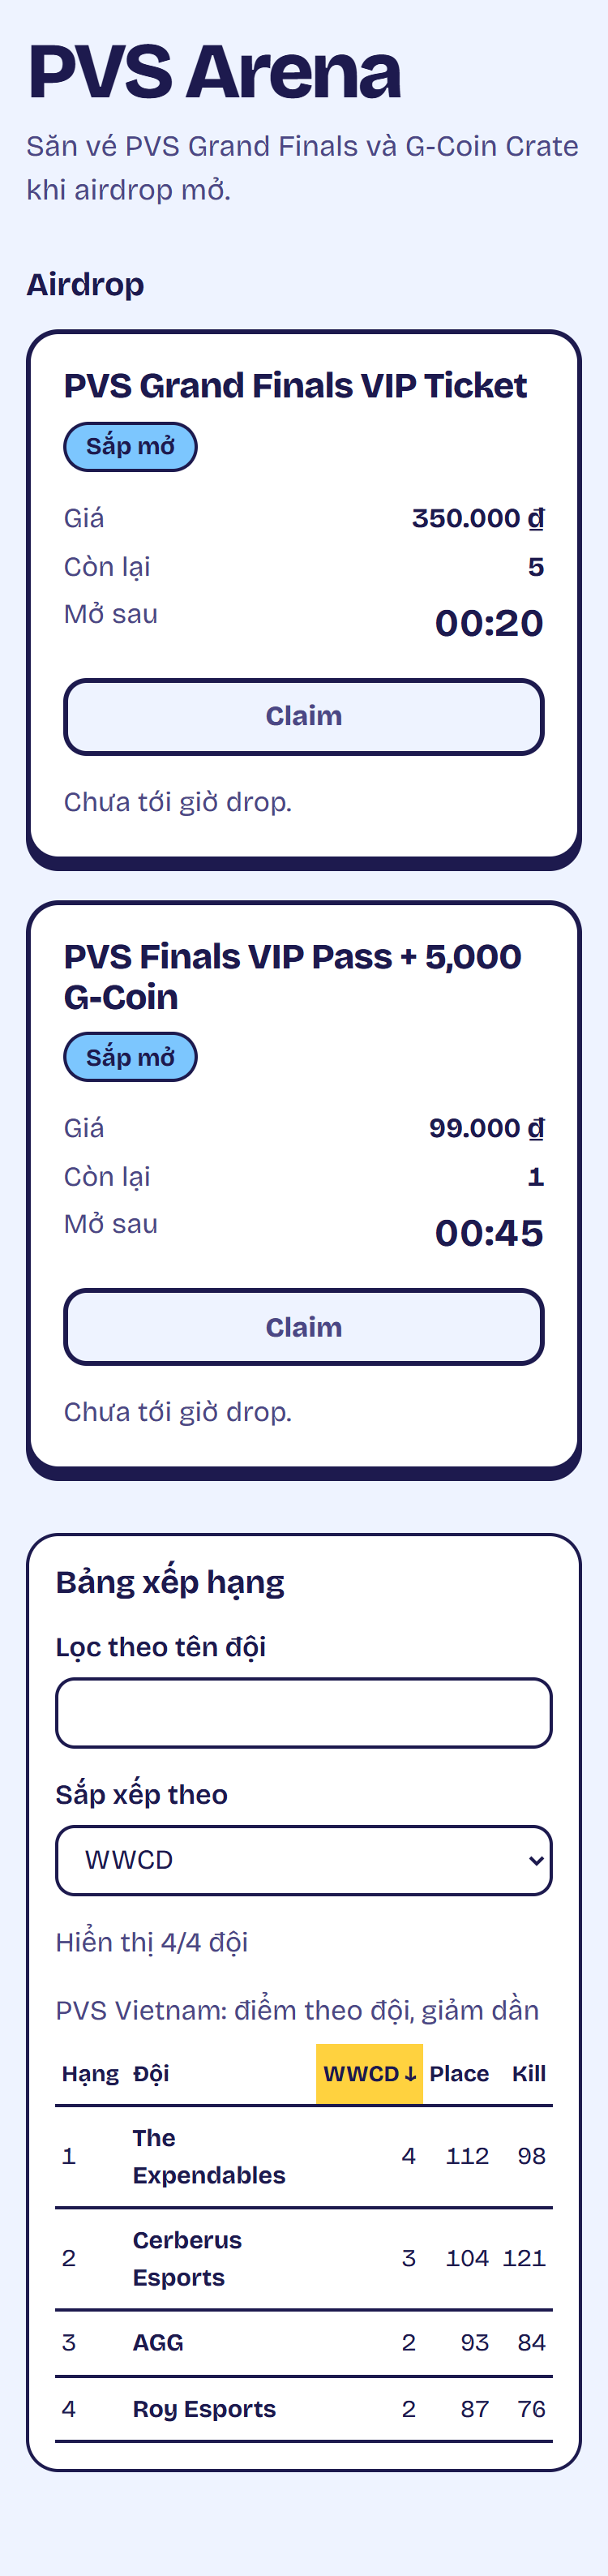
\includegraphics[width=0.3\textwidth,trim=0 1000bp 0 0,clip]{images/hw3_375.png}
    \caption{375 px (top of the page): countdown, VND price, disabled Claim with a reason}
    \label{fig:hw3-375}
\end{figure}

\evfig{hw3_409.png}{0.3}{Claim rejected with 409: stock returns to its old value and an alert explains why}{fig:hw3-409}
\evfig{hw3_lighthouse.png}{0.9}{Lighthouse: Performance 100, Accessibility 100, Best Practices 100}{fig:hw3-lh}
\evfig{hw3_a11y.png}{0.9}{Accessibility tree of the Claim button}{fig:hw3-a11y}

\section{Verification}

\begin{table}[H]
\centering
\begin{tabular}{L{5.5cm} L{7.5cm}}
\toprule
\textbf{Check} & \textbf{Result} \\
\midrule
\texttt{npm test} & 7 files, 61 tests pass \\
\texttt{npm run lint} & Clean \\
Hidden tab 330 s & Displayed 04:29, drift 0 s (before and after wake) \\
409 rollback & Stock 1 $\rightarrow$ 0 $\rightarrow$ 1, alert shown \\
Horizontal scroll, 320 and 375 px & None \\
Contrast & 14/14 pairs pass, lowest 6.24:1 \\
Claim transition & 0.07 s; 0 s with reduced motion \\
Lighthouse & 100 / 100 / 100 \\
\bottomrule
\end{tabular}
\caption{Homework 3 results}
\label{tab:hw3-verify}
\end{table}

Not done: screen reader test; Lighthouse SEO was not run.

\section{AI Failure Audit}

\begin{itemize}
    \item Test runner reported as flaky''; the real cause was running \texttt{npm test} from the wrong folder (error 6).
    \item Countdown \texttt{<output>} was a live region announcing every second (error 7).
\end{itemize}

\section{Source Code}

\begin{center}
    \href{https://github.com/Prosperum26/24520626_QuangPhuHung_MSIS207_Lab03/tree/main/src/homeworks/KraftonPubgVnArena}
    {\textbf{View Homework 3 on GitHub}}

    \href{https://github.com/Prosperum26/24520626_QuangPhuHung_MSIS207_Lab03/blob/main/AI_FAILURE_AUDIT.md}
    {\textbf{View AI failure audit on GitHub}}
\end{center}
